\documentclass[addpoints,12pt]{exam}
\usepackage[spanish]{babel}
%\usepackage[latin1]{inputenc}
\usepackage[utf8x]{inputenc}
\usepackage{graphicx}
\pagestyle{empty}
\begin{document}
\begin{center}
\fbox{\fbox{\parbox{5.5in}{\centering {\LARGE EXAMEN TIPO B}\\Sigue las intrucciones que marca el ejercicio, no solo para la realización del mismo sino también para la entrega.\\\emph{No se permite ningun documento de ayuda, excepto los aportados por el profesor}\\Se permite la realización del ejercicio en Eclipse o Netbeans utilizando un workspace vacío y crea un \emph{package} denominado \emph{\textit{segundaevaluacion}}}}}
\end{center}
\vspace{0.1in}
%\makebox[\textwidth]{Nombre:\enspace\hrulefill}

\begin{questions}

\question Crea una clase denominada \emph{Ejercicio1} que incorpore la librería externa \emph{auxiliar.jar}. Crea dos objetos de tipo \emph{Palabra} y comprueba el funcionamiento de todos los métodos que contiene dicha clase \emph{Palabra} en el diagrama UML.
\\
Posteriormente crea un jar ejecutable denominado \emph{ejercicio1.jar}\\
\vspace{0.3cm}
\\
Criterios de evaluación:
\begin{description}
\item[1 pto.] Funcionamiento correcto de la clase \emph{Ejercicio1}.
\item[1 pto.] Funcionamiento correcto de la clase \emph{ejercicio1.jar}.
\end{description}
En el caso que no seas capaz de incorporar dicha biblioteca, puedes diseñar la parte que te corresponde en una clase aparte y posteriormente realizar el ejercicio tal y como se te pide. En este caso la puntuación del ejercicio es de solo 1 punto y siempre y cuando esté funcionando correctamente. 
\begin{figure}[h]
\centering
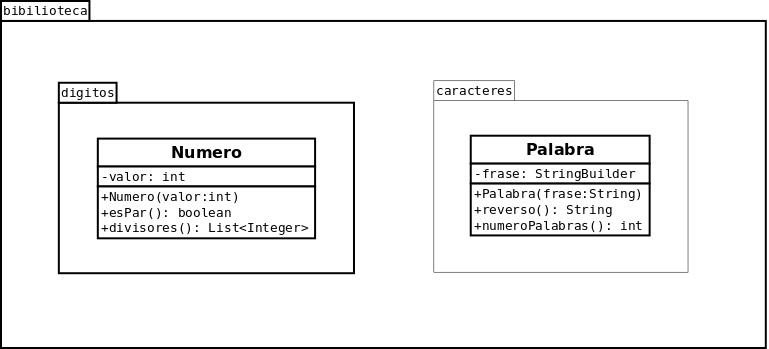
\includegraphics[scale=0.3]{examen.png}
\caption{Diagrama UML para el ejercicio 1}
\end{figure}
\question Crea una clase denominada \emph{Ejercicio2} que cree una lista de tipo \emph{ArrayList} de objetos de tipo \emph{Telefono}. Para la creación de objetos de tipo \emph{Telefono} usarás un \emph{Scanner} que lea los atributos y los añadirá a la lista, la única objeción que se plantea es que no puede haber dos teléfonos con el mismo modelo, por lo que tendrás que consultar en la lista para que no se añadan dos modelos iguales a la misma o bien sobeescribir los métodos \emph{equals} y \emph{hascode}, indicando que dos objetos \emph{Telefono} son iguales cuando coincide el modelo. Para comprobar el correcto funcionamiento, muestra la lista en pantalla.\\
Tanto el modelo como la MAC se crearan de manera aleatoria usando los correspondientes métodos que aporta la clase \emph{Telefono}\\
La MAC consta de 12 cifras o letras, agrupadas de dos en dos y separadas por dos puntos. Ejemplo: 00:12:fe:dd:11:12. Pueden contener cualquier cifra del 0 al 9 y las letras a, b, c, d, ó f.\\
En cuanto al modelo su formato es una letra en mayúscula y dos cifras. Ejemplos: A23, Z65, O23, \dots\\
Posteriormente crea un \emph{StringBuilder} que recoja los modelos usando como separador una coma: A23, Z65, O23, Q33. Observa que tanto al final como al principio no debe haber un espacio en blanco. Para comprobar su funcionamiento imprime dicho \emph{StringBuilder}.
Para esta última parte puedes añadir a la clase \emph{Telefono} algún \emph{getter} que pudiera hacerte falta.\\
Para acabar el \emph{Scanner} usa la palabra \emph{quit} cuando intentes leer el atributo \emph{nombre}.\\
También crearás un jar ejecutable denominado \emph{ejercicio2.jar} así como la documentación en \emph{javadoc} de la clase \emph{Telefono}. Esta debe aparecer en el \emph{workspace}
\vspace{0.3cm}
\\
Criterios de evaluación:
\begin{description}
\item[2 ptos.] Funcionamiento correcto de la clase \emph{Telefono}.
\item[1 pto.] Funcionamiento correcto del clase \emph{Scanner}.
\item[1 pto.] Creación de lista correctamente.
\item[1 pto.] Creación del StringBuilder.
\item[0.5 ptos.] Creación del jar ejecutable.
\item[0.5 ptos.] Creación de la documentación. 
\end{description}
\begin{figure}[h]
\centering
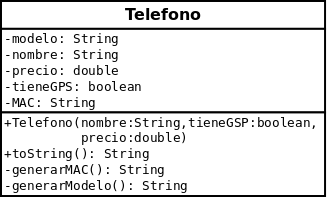
\includegraphics[scale=0.5]{telefono.png}
\caption{Diagrama UML para el ejercicio 2}
\end{figure}
\end{questions}
%\newpage
\textbf{Formato del fichero de subida:} se subirá un archivo comprimido de la siguiente forma nombreApellidos.tar.gz o nombre.Apellidos.zip. En el debes incluir:
\begin{itemize}
\item El \emph{workspace} donde has realizado el examen. 
\item El fichero jar ejecutable del primer ejercicio.
\item El fichero jar ejecutable del segundo ejercicio.
\end{itemize}


\end{document}
